\documentclass[oneside,final,14pt]{extreport}
\usepackage[utf8]{inputenc}
\usepackage[russianb]{babel}
\usepackage{vmargin}
\usepackage{amsmath}
\usepackage{amsfonts}
\usepackage{amssymb}
\usepackage{graphicx}
\usepackage[usenames]{color}
\setpapersize{A4}
\setmarginsrb{2cm}{1.5cm}{1cm}{1.5cm}{0pt}{0mm}{0pt}{13mm}
\usepackage{indentfirst}
\sloppy



\begin{document}

\section* {
\begin{centering}
	Вычислительные Методы\\
	Отчёт по лабораторной работе №2\\
\end{centering}
}


\begin{center}
	Выполнил студент группы КЭ-201 Гордеев Александр\\
	Вариант № 4\\
	Метод простой итерации\\
\end{center}


{\bfseries Данные:}

$x = \arctg{3x}$

$\varepsilon = 0.001$\\


{\bfseries 1. Отделяем корни уравнения}

Строим график и находим граничные точки

\begin{center}
	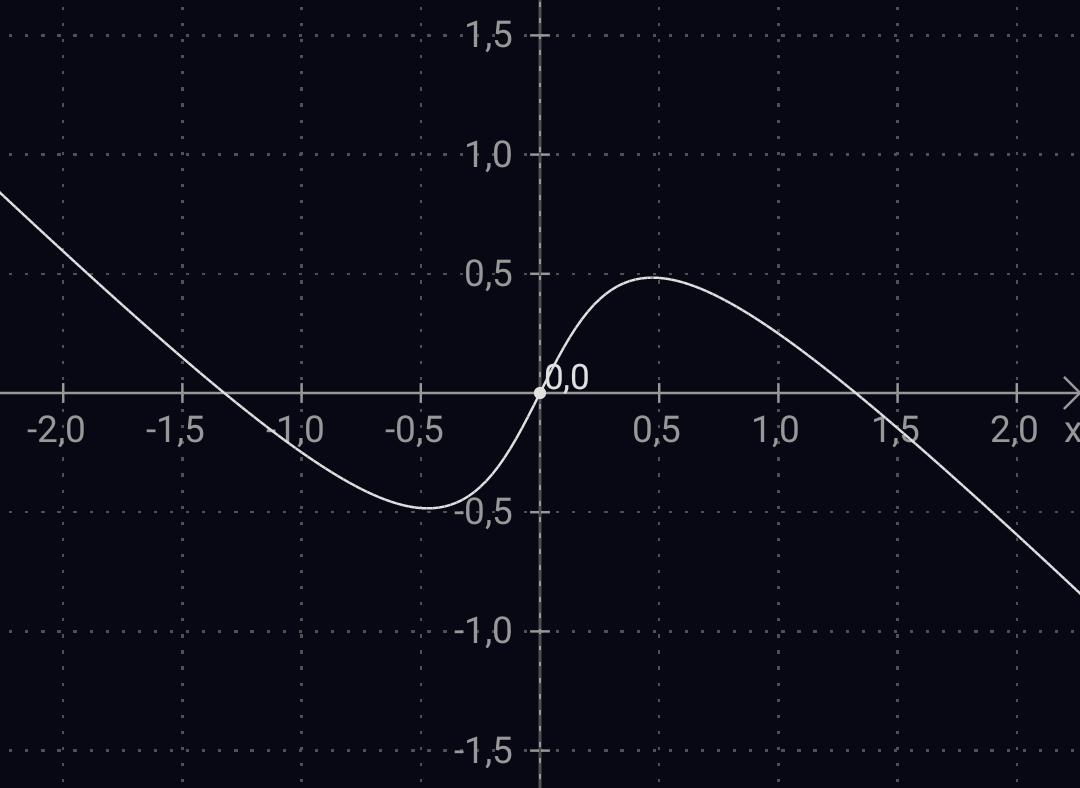
\includegraphics[scale=0.26]{lab2.png} \\
	График функции $f(x) = \arctg{3x} - x$
\end{center}

Очевидный корень $x_1 = 0$

Приближенные корни $x_0 = \pm 1$\\


{\bfseries 2. Уравнение пригодное для итерации}

$f(x) = \arctg{3x}$\\


{\bfseries 3. Проверка условия сходимости}

$f'(x) = \frac{\displaystyle 3}{\displaystyle 9x^2 + 1}$\\

1. $q = \lvert f'(x_0) \rvert \leqslant 1$

\hspace{5.3mm}$q = \lvert f'(\pm 1) \rvert = \bigg | \frac{\displaystyle 3}{\displaystyle 9 * (\pm 1)^2 + 1} \bigg | = 0.3 \leqslant 1$\\

2. $\lvert f(x_0) - x_0 \rvert \leqslant (1 - q) * \delta$

\hspace{5.3mm}$\lvert \arctg(3 * (\pm 1)) - (\pm 1) \rvert \leqslant (1 - 0.3) * 0.5$

\hspace{5.3mm}$\lvert \pm 0.249 \rvert = 0.249 \leqslant 0.35$\\

Все условия сходимости выполняются.


{\bfseries 4. Результат работы программы}

Найденные корни уравнения:

$x_1 = 0$

$x_2 = -1.324$

$x_3 = 1.324$\\


{\bfseries 5. Проверка корней}

Подставим корни в исходное уравнение $x = \arctg{3x}$

$x_1 = 0$

$0 = \arctg{0}$

$0 = 0$\\

$x_2 = -1.324$

$-1.324 = \arctg(3 * (-1.324))$

$-1.324 = -1.324$\\

$x_3 = 1.324$

$1.324 = \arctg(3 * 1.324)$

$1.324 = 1.324$\\

Все корни прошли проверку.\\

Итоговый ответ:

$x = 0; \pm 1.324$

\end{document}
